\documentclass[11pt]{amsart}
\usepackage[T1]{fontenc}
\usepackage[utf8]{inputenc}
\usepackage{lmodern}
\usepackage{amsmath,amssymb,amsthm}
\usepackage{graphicx}
\usepackage[dvipsnames]{xcolor}
\usepackage{booktabs}
\usepackage[margin=1.15in]{geometry}
\usepackage[colorlinks=true,linkcolor=blue!50!black,citecolor=blue!50!black,urlcolor=blue!50!black]{hyperref}

\newtheorem{conjecture}{Heuristic prediction}
\newtheorem{lemma}{Lemma}
\theoremstyle{remark}
\newtheorem{remark}{Remark}

\newcommand{\Sing}{\mathfrak{S}}
\newcommand{\cH}{\mathcal{H}}
\DeclareMathOperator{\li}{li}

\title[Zeros of $\zeta$ and $L$-functions in prime pairs and triplets]{The zeros of $\zeta$ and of Dirichlet $L$-functions in the fluctuations of prime pairs and prime triplets: a numerical study}

\author{Antony Geremia}
\address{Independent researcher, France}

\date{November 2026}
\subjclass[2020]{11N05, 11N13, 11M26, 11Y35}
\keywords{prime $k$-tuples, Hardy--Littlewood conjecture, explicit formula, Dirichlet $L$-functions, twin primes, matched filter}

\begin{document}

\begin{abstract}
Let $W_\cH(x)=\sum \prod_i \log(p+h_i)$ count, with logarithmic weights, the primes $p\le x$ for which every $p+h_i$ is prime, for an admissible pattern $\cH=(h_1,\dots,h_k)$. The Hardy--Littlewood conjecture predicts $W_\cH(x)\sim\Sing(\cH)\,x$. A first-order heuristic, in which each member of the pattern carries the local fluctuation of the primes in its residue class, predicts that the oscillating part of $W_\cH(x)-\Sing(\cH)x$ is $\Sing(\cH)\sum_\chi c_\chi(\cH)\,\psi(x,\chi)$, with explicit coefficients $c_\chi(\cH)$ given by averages of characters over admissible residue classes. In particular the zeros of $\zeta$ enter with weight $k\,\Sing(\cH)$, and the zeros of $L(s,\chi)$ enter with a weight whose sign depends on~$\cH$.
We test this prediction numerically, with no fitted parameter, using an exact sieve up to $10^{10}$ (and up to $10^{12}$ for $h=2,4,6$), and a matched filter that projects the fluctuations onto the explicit templates $(\psi(x)-x)/\sqrt{x}$ and $\psi(x,\chi)/\sqrt{x}$ in the frequency band $50\le\gamma\le 6000$. For the thirty gaps $h=2,\dots,60$, the $\zeta$ term is found at $0.98\pm0.04$ times its predicted size, and twin primes alone at $1.09\pm0.15$ ($7\sigma$). The real character modulo $5$ appears at $1.01\pm0.07$ times its prediction ($14\sigma$), with the predicted sign for each of the $24$ gaps not divisible by~$5$. For $50$ triplet patterns $(0,a,b)$, $b\le 24$, the $\zeta$ term is found at $0.98\pm0.07$, and the odd character modulo~$3$, which cannot appear for pairs, appears at $0.91\pm0.13$ ($7\sigma$), with opposite signs for mirror patterns such as $(0,2,6)$ and $(0,4,6)$. Characters with vanishing predicted coefficient are consistent with noise. All errors are obtained by time slides and account for the correlations between patterns. Nothing here is proved; the results are numerical evidence for a heuristic.
\end{abstract}

\maketitle

\section{Introduction}

For an admissible pattern $\cH=(h_1,\dots,h_k)$ of distinct integers ($h_1=0$), the prime $k$-tuples conjecture of Hardy and Littlewood~\cite{HL} predicts
\begin{equation}\label{eq:HL}
W_\cH(x):=\sum_{\substack{p\le x\\ p+h_i\ \text{prime}\ \forall i}}\ \prod_{i=1}^k\log(p+h_i)\ \sim\ \Sing(\cH)\,x,
\qquad
\Sing(\cH)=\prod_p\Bigl(1-\frac{\nu_p(\cH)}{p}\Bigr)\Bigl(1-\frac1p\Bigr)^{-k},
\end{equation}
where $\nu_p(\cH)$ is the number of residue classes modulo $p$ occupied by $\cH$. Even the case $k=2$, $\cH=(0,2)$ (twin primes) is open. This note is not about the main term, but about the \emph{fluctuations} $W_\cH(x)-\Sing(\cH)x$, which are of size about $\sqrt{x}$ (times logarithms).

For $k=1$, the fluctuations of the primes are described exactly by the explicit formula $\psi(x)-x=-\sum_\rho x^\rho/\rho+O(\log x)$, and in residue classes by $\psi(x,\chi)=\sum_{n\le x}\chi(n)\Lambda(n)=-\sum_{\rho_\chi}x^{\rho_\chi}/\rho_\chi+\dots$ for non-principal $\chi$ (see e.g.~\cite{Davenport}). It is natural to expect that the fluctuations of prime patterns contain the same oscillations. For pairs, averaged over the gap $h$, such a formula was proposed and tested up to $10^{12}$ by Korevaar and te Riele~\cite{KtR}; related averaged formulas for the Goldbach problem go back to Fujii~\cite{Fujii}, and versions in arithmetic progressions, where zeros of Dirichlet $L$-functions appear, are studied in~\cite{Suzuki,BHMS}. In the opposite direction, the correlations of the zeros of $\zeta$ contain the Hardy--Littlewood constants~\cite{BK,KS}.

Here we look at each pattern separately and at each character separately. A one-line heuristic (Section~\ref{sec:heur}) predicts the size \emph{and the sign} of every oscillating term, without any free parameter. Two features make the test sharp:
\begin{itemize}
\item the coefficient of $\psi(x,\chi)$ changes sign with the pattern, so it disappears from any average over patterns and must be detected pattern by pattern;
\item for pairs the coefficient vanishes for every odd character (Lemma~\ref{lem:pairs}), while for triplets it does not: the odd character modulo~$3$ must appear in triplets, with opposite signs for a pattern and its mirror image (Lemma~\ref{lem:mirror}).
\end{itemize}
Single patterns are noisy: for twin primes, the counting noise of $W_2$ is about twenty times larger than the predicted oscillation in a naive spectrogram. We use instead a matched filter, as in gravitational-wave searches: the expected waveform is known exactly (it is computed from the primes themselves, or from the zeros), and we project the data on it in a wide frequency band. Noise is estimated by time slides.

We stress that nothing below is a theorem. The prediction is heuristic, and the numerical results are evidence for it, in a limited range. We have not found the pattern-by-pattern and character-by-character prediction stated in this form in the literature, but it follows from standard heuristics and may well be known to experts.

\section{The heuristic prediction}\label{sec:heur}

Fix a modulus $q$ and let $A_q(\cH)$ be the set of residue classes $a\bmod q$ such that $\gcd(a+h_i,q)=1$ for all $i$. In the Hardy--Littlewood model, primes $p$ completing the pattern are equidistributed among the classes of $A_q(\cH)$. Near $t$, the density of primes in a class $r$ coprime to $q$ is, by orthogonality,
\[
\frac{1}{\varphi(q)}\Bigl(1+\sum_{\chi\bmod q}\bar\chi(r)\,\delta_\chi(t)\Bigr),
\qquad \delta_\chi(t)=\frac{d}{dt}\bigl(\psi(t,\chi)-\mathbf 1_{\chi=\chi_0}\,t\bigr),
\]
understood as a distribution whose oscillating part is $-\sum_{\rho_\chi}t^{\rho_\chi-1}$. If each member $p+h_i$ of the pattern carries independently the fluctuation of its own class, the density of patterns is multiplied by $\prod_i(1+\sum_\chi\bar\chi(a+h_i)\delta_\chi)\approx 1+\sum_\chi\bigl(\sum_i\bar\chi(a+h_i)\bigr)\delta_\chi$. Averaging over $a\in A_q(\cH)$ and integrating gives the following.

\begin{conjecture}\label{conj}
Let $u=\log x$ and $E_\cH(u)=(W_\cH(x)-\Sing(\cH)x)/\sqrt{x}$. In any fixed band of frequencies $\gamma$ (in the variable~$u$), and up to a noise term,
\begin{equation}\label{eq:pred}
E_\cH(u)\ \approx\ \Sing(\cH)\sum_{\chi\bmod q} c_\chi(\cH)\,\frac{\psi(x,\chi)-\mathbf 1_{\chi=\chi_0}x}{\sqrt{x}},
\qquad
c_\chi(\cH)=\frac{1}{|A_q(\cH)|}\sum_{a\in A_q(\cH)}\ \sum_{i=1}^k\bar\chi(a+h_i).
\end{equation}
\end{conjecture}

For the principal character, $c_{\chi_0}(\cH)=k$, so the zeros of $\zeta$ enter with weight $k\,\Sing(\cH)$: this is the expansion $(1+\varepsilon)^k\approx 1+k\varepsilon$. For several moduli one may combine the characters by the Chinese remainder theorem; below we only use one character at a time, and fit all templates jointly. For a complex character, $\chi$ and $\bar\chi$ together contribute $2\Sing\,(\operatorname{Re}c_\chi\,\operatorname{Re}\psi(x,\chi)-\operatorname{Im}c_\chi\,\operatorname{Im}\psi(x,\chi))$.

The prediction ignores the products of fluctuations (second order), the prime powers, and the correlations between the members of the pattern beyond the singular series. Its content is the size and sign of the first-order oscillating terms. The following elementary facts make it easy to test.

\begin{lemma}\label{lem:pairs}
Let $\cH=(0,h)$ and let $q$ be a prime not dividing $h$. Then $c_\chi(\cH)=-2\bar\chi(h)/(q-2)$ if $\chi\ne\chi_0$ is even, and $c_\chi(\cH)=0$ if $\chi$ is odd. If $q\mid h$, then $c_\chi(\cH)=0$ for $\chi\ne\chi_0$.
\end{lemma}

\begin{proof}
If $q\nmid h$, $A_q=\{a: a\not\equiv 0,-h\}$ has $q-2$ elements. Since $\sum_{a\bmod q}\bar\chi(a)=0$, we get $\sum_{a\in A_q}\bar\chi(a)=-\bar\chi(-h)$ and $\sum_{a\in A_q}\bar\chi(a+h)=-\bar\chi(h)$, whose sum is $-\bar\chi(h)(1+\chi(-1))$. If $q\mid h$, both sums are over all nonzero classes and vanish.
\end{proof}

\begin{lemma}\label{lem:mirror}
Let $\cH^*=h_{\max}-\cH$ be the mirror image of $\cH$. Then $c_\chi(\cH^*)=\chi(-1)\,c_\chi(\cH)$. In particular $c_\chi(\cH)=0$ for odd $\chi$ whenever $\cH^*$ is a translate of $\cH$, as for every pair.
\end{lemma}

\begin{proof}
The map $a\mapsto -a-h_{\max}$ is a bijection $A_q(\cH)\to A_q(\cH^*)$, and $-a-h_{\max}+(h_{\max}-h_i)=-(a+h_i)$, so each character value is multiplied by $\bar\chi(-1)=\chi(-1)$.
\end{proof}

\begin{remark}
For triplets the odd character $\chi_3$ modulo $3$ need not vanish. The pattern $(0,2,6)$ forces $p\equiv 2\pmod 3$, so its members lie in the classes $2,1,2$ and $c_{\chi_3}=-1$; its mirror image $(0,4,6)$ forces $p\equiv1$ and gives $c_{\chi_3}=+1$. On the other hand, a pattern of even integers imposes nothing modulo $4$ or $8$ on an odd prime, so $c_\chi=0$ for the characters modulo $4$ and $8$, and for the real character modulo $12$; these serve as controls.
\end{remark}

\section{Data and method}\label{sec:method}

\subsection*{Sieve}
We sieved all integers up to $N=10^{10}$ (in Python with NumPy, and independently in C), and recorded on a grid $x_j=\lfloor e^{u_j}\rfloor$, $u_j=\log 10^3+0.0005\,j$, the quantities $\psi(x)$, $\psi(x,\chi)$ for the characters listed below, and $W_\cH(x)$ for the patterns studied. Checks: $\pi(10^{10})=455\,052\,511$ and $27\,412\,679$ twin prime pairs below $10^{10}$, the known values. A faster C sieve extends $W_h$ for $h=2,4,6$ to $10^{12}$, reproducing the known count of $1\,870\,585\,220$ twin pairs below $10^{12}$~\cite{OEIS}. The last grid point below $10^{10}$ is $x=9\,999\,043\,536$.

Characters used: the real characters $\chi_3,\chi_4,\chi_5,\chi_8,\chi_{12},\chi_{13}$ (moduli $3,4,5,8,12,13$; $\chi_3,\chi_4$ are odd, the others even), the complex odd character $\chi_5'$ modulo $5$ with $\chi_5'(2)=i$, and the cubic character $\chi_7$ modulo $7$ (even).

\subsection*{Matched filter}
Let $f(u)=(\psi(x)-x)/\sqrt x$ and $g_\chi(u)=\psi(x,\chi)/\sqrt x$ (real and imaginary parts as separate templates when $\chi$ is complex). On the interval $9\le u\le\log x_{\max}$ we apply a Hann window, take the discrete Fourier transform, and keep the frequencies $50\le\gamma\le6000$ (this band contains $5\,588$ zeros of $\zeta$). Below $\gamma=50$ the counting noise of a single pattern dominates. For each pattern $\cH$ we compute the coefficients $\hat\beta_\cH$ of the least-squares fit of the filtered $E_\cH$ by all filtered templates jointly, and compare them with the predictions~\eqref{eq:pred}. No parameter is adjusted.

\subsection*{Noise: time slides}
The templates are shifted cyclically along $u$ by $50$ offsets between $0.75$ and $13$ (in units of~$u$), which destroys the phase coherence with the true oscillations, and the fit is repeated. The standard deviation $\sigma_\cH$ of the $50$ shifted coefficients is the noise of $\hat\beta_\cH$.

\subsection*{Combining patterns}
For a template with predictions $\pi_\cH$, we estimate a common ratio ``measured/predicted''
$\kappa=\sum_\cH\hat\beta_\cH\pi_\cH\sigma_\cH^{-2}\big/\sum_\cH\pi_\cH^2\sigma_\cH^{-2}$.
The patterns share their primes, so their noises are correlated, and the naive error $(\sum\pi_\cH^2\sigma_\cH^{-2})^{-1/2}$ is too small (by a factor of about $2$ for the $\zeta$ template). We therefore recompute $\kappa$ with the shifted coefficients for each of the $50$ time slides and use the standard deviation of these values; we report the larger of the two errors. For templates whose prediction is $0$ for every pattern, we report $\chi^2=\sum(\hat\beta_\cH/\sigma_\cH)^2$ and compare it with the distribution of the same statistic over the time slides.

\section{Results for pairs}

The thirty gaps $h=2,4,\dots,60$ all follow~\eqref{eq:HL} to within $0.016\%$ at $10^{10}$. Table~\ref{tab:pairs} and Figure~\ref{fig:pairs} give the coefficients.

\begin{itemize}
\item \emph{The $\zeta$ term.} Combining the thirty gaps, $\kappa_\zeta=0.98\pm0.04$ ($22\sigma$). Each gap separately is consistent with~$1$; gaps with $6\mid h$, whose $\Sing(h)$ is twice as large, carry an oscillation twice as large.
\item \emph{Twin primes alone.} For $h=2$, $\hat\beta/2\Sing(2)=1.09\pm0.15$ ($7\sigma$); none of the $50$ time slides exceeds $0.37$.
\item \emph{Characters.} $\chi_5$: $\kappa=1.01\pm0.07$ ($14\sigma$), with the predicted sign ($+2/3$ for $h\equiv\pm2$, $-2/3$ for $h\equiv\pm1\bmod 5$) for each of the $24$ gaps not divisible by $5$, and values consistent with $0$ for the six multiples of $5$. Cubic $\chi_7$ (real and imaginary parts together): $1.08\pm0.08$ ($14\sigma$). $\chi_{13}$, whose coefficients are small ($\pm2/11$): $0.93\pm0.17$ ($5\sigma$).
\item \emph{Controls.} The odd characters $\chi_3,\chi_4,\chi_5'$ and the even characters $\chi_8,\chi_{12}$, for which the prediction vanishes, give $\chi^2$ between $26$ and $37$ for $30$ gaps, while the time slides give $31\pm9$.
\end{itemize}

\subsection*{A blind test beyond $10^{10}$}
The prediction being fixed, we counted the new pairs with $10^{10}<p\le10^{12}$ for $h=2,4,6$. Since $\psi(x)$ was not computed that far, the template was built from the zeros, $f(u)=-2\operatorname{Re}\sum_{\gamma<7000}e^{i\gamma u}/(\tfrac12+i\gamma)$, using $138\,069$ zeros computed with the Riemann--Siegel formula; on $[10^3,10^{10}]$ its correlation with the sieve template in the band is $0.991$. On the new data alone: $0.61\pm0.31$ ($h=2$), $1.07\pm0.31$ ($h=4$), $1.05\pm0.29$ ($h=6$), and $0.91\pm0.17$ combined ($5\sigma$). The signal-to-noise ratio does not grow much with $x$: the filtered counting noise of $W_2/\sqrt x$ grows roughly like $\log x$ (from $0.77$ to $1.35$ between $10^5$ and $10^8$), while the oscillation keeps a constant size. For twin primes alone, the significance reaches about $8\sigma$ near $x=5\cdot10^8$ and is $6$--$7\sigma$ from $10^{10}$ to $5\cdot10^{11}$.

\begin{figure}[t]
\centering
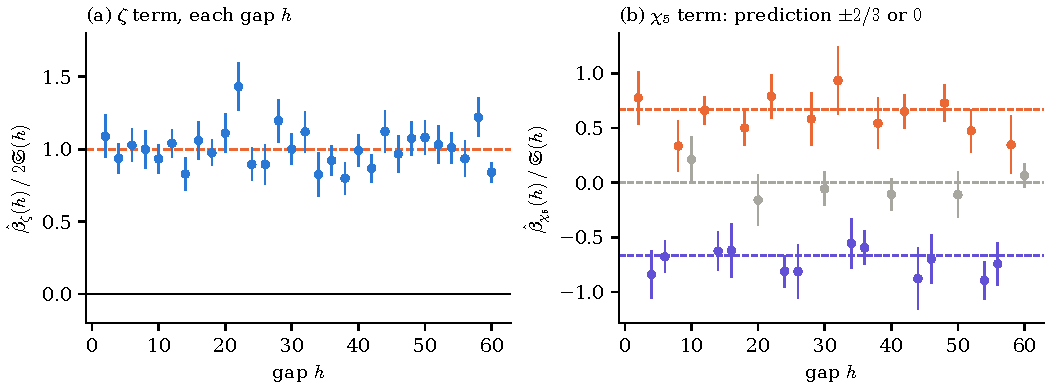
\includegraphics[width=\textwidth]{fig_pairs.pdf}
\caption{Pairs $(p,p+h)$ up to $10^{10}$. (a) Coefficient of the $\zeta$ template divided by its prediction $2\Sing(h)$. (b) Coefficient of the $\chi_5$ template divided by $\Sing(h)$; dashed lines: predictions $+2/3$ (orange), $-2/3$ (violet), $0$ for $5\mid h$ (grey). Error bars: one standard deviation from time slides.}
\label{fig:pairs}
\end{figure}

\begin{table}[t]
\centering\small
\caption{Pairs up to $10^{10}$: combined ratio $\kappa$ (measured/predicted) for each template. For controls (prediction $0$ for all gaps), $\chi^2$ for $30$ gaps and its mean $\pm$ standard deviation over the time slides.}
\label{tab:pairs}
\begin{tabular}{lll}
\toprule
template & prediction & result\\
\midrule
$\zeta$ & $2\Sing(h)$ & $\kappa=0.980\pm0.044$\\
$\chi_5$ (even) & $\mp\tfrac23\Sing(h)$ or $0$ & $\kappa=1.006\pm0.070$\\
$\chi_7$ cubic (even), Re and Im & $-\tfrac25\Sing(h)\bar\chi_7(h)$ & $\kappa=1.083\pm0.079$\\
$\chi_{13}$ (even) & $\mp\tfrac{2}{11}\Sing(h)$ or $0$ & $\kappa=0.925\pm0.172$\\
\midrule
$\chi_3$ (odd) & $0$ & $\chi^2=28.0$ \quad(slides $30.5\pm7.8$)\\
$\chi_4$ (odd) & $0$ & $\chi^2=37.1$ \quad(slides $31.1\pm7.3$)\\
$\chi_5'$ (odd), Re / Im & $0$ & $\chi^2=26.3\ /\ 30.7$ \quad(slides $31.1\pm7.9\ /\ 30.6\pm10.1$)\\
$\chi_8$ (even) & $0$ & $\chi^2=25.9$ \quad(slides $31.2\pm10.2$)\\
$\chi_{12}$ (even) & $0$ & $\chi^2=34.0$ \quad(slides $30.8\pm10.5$)\\
\bottomrule
\end{tabular}
\end{table}

\section{Results for triplets}

We studied the $50$ admissible triplet patterns $(0,a,b)$ with $a<b\le24$ even (admissibility only matters modulo $2$ and $3$), and the quadruplet $(0,2,6,8)$; in total about $190$ million triplets up to $10^{10}$.

\begin{itemize}
\item \emph{Hardy--Littlewood.} All $50$ counts agree with $\Sing(\cH)\int_2^x dt/\prod_i\log(t+h_i)$ to within $0.11\%$. For instance there are $2\,713\,122$ triplets $(p,p+2,p+6)$ with $p\le 9\,999\,043\,536$, against $2\,715\,062$ predicted ($\Sing=2.8582$).
\item \emph{The $\zeta$ term} (prediction $3\Sing(\cH)$): $\kappa=0.98\pm0.07$ ($14\sigma$).
\item \emph{The odd character $\chi_3$.} The prediction is $-\Sing$ for $22$ patterns, $+\Sing$ for $22$ others, and $0$ for the $6$ patterns made of multiples of $6$. We find $\kappa=0.91\pm0.13$ ($7\sigma$). Individual patterns are noisy: $(0,2,6)$ gives $-0.70\pm0.88$ and its mirror image $(0,4,6)$ gives $+2.20\pm1.07$ (in units of $\Sing$).
\item \emph{Other characters.} $\chi_5$: $1.01\pm0.10$ ($10\sigma$); cubic $\chi_7$: $0.92\pm0.13$ ($7\sigma$); the odd complex character $\chi_5'$, whose prediction is nonzero for $20$ of the $50$ patterns: $0.92\pm0.29$ ($3\sigma$); $\chi_{13}$: $0.64\pm0.39$, inconclusive.
\item \emph{Controls.} $\chi_4,\chi_8,\chi_{12}$ (prediction $0$ for every triplet): $\chi^2=45.4$, $51.4$, $53.9$ for $50$ patterns, against $51.5\pm11.0$, $52.1\pm9.8$, $51.8\pm13.4$ over the time slides.
\item \emph{The quadruplet} $(0,2,6,8)$: $180\,517$ up to the same bound, $0.3\%$ below the prediction; its $\zeta$ coefficient, $1.9\pm0.8$ times $4\Sing$, is too noisy to be informative.
\end{itemize}

The naive error for the $\zeta$ template, which treats the $50$ patterns as independent, would be $\pm0.034$ ($29\sigma$); the time-slide error, which accounts for their correlation, is twice as large.

\begin{figure}[t]
\centering
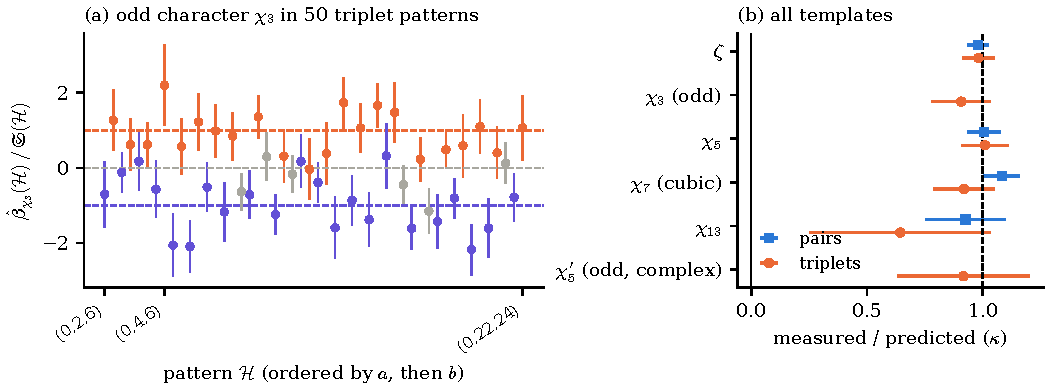
\includegraphics[width=\textwidth]{fig_triplets.pdf}
\caption{(a) Triplet patterns $(0,a,b)$, $b\le 24$, up to $10^{10}$: coefficient of the $\chi_3$ template divided by $\Sing(\cH)$. Predictions: $-1$ (violet), $+1$ (orange), $0$ (grey). (b) Combined ratio measured/predicted for every template with a nonzero prediction, for pairs (squares) and triplets (circles); $\chi_3$ and $\chi_5'$ have zero prediction for pairs.}
\label{fig:triplets}
\end{figure}

\begin{table}[t]
\centering\small
\caption{Selected triplet patterns up to $x=9\,999\,043\,536$: counts, Hardy--Littlewood prediction, singular series, and the coefficients of the $\zeta$ template (divided by $3\Sing$) and of the $\chi_3$ template (divided by $\Sing$), with the prediction $c_{\chi_3}$.}
\label{tab:triplets}
\begin{tabular}{lrrrcrr}
\toprule
$\cH$ & count & HL prediction & $\Sing(\cH)$ & $\zeta$ & $c_{\chi_3}$ & $\chi_3$\\
\midrule
$(0,2,6)$ & 2\,713\,122 & 2\,715\,062 & 2.8582 & $0.93\pm0.28$ & $-1$ & $-0.70\pm0.88$\\
$(0,4,6)$ & 2\,712\,007 & 2\,715\,062 & 2.8582 & $1.86\pm0.34$ & $+1$ & $+2.20\pm1.07$\\
$(0,2,8)$ & 2\,715\,324 & 2\,715\,062 & 2.8582 & $0.79\pm0.33$ & $+1$ & $+1.26\pm0.81$\\
$(0,6,8)$ & 2\,715\,436 & 2\,715\,061 & 2.8582 & $0.73\pm0.34$ & $-1$ & $-1.17\pm0.78$\\
$(0,6,12)$ & 5\,427\,503 & 5\,430\,121 & 5.7165 & $0.96\pm0.22$ & $0$ & $-0.63\pm0.49$\\
$(0,12,24)$ & 5\,428\,556 & 5\,430\,119 & 5.7165 & $0.89\pm0.20$ & $0$ & $-1.15\pm0.60$\\
$(0,22,24)$ & 3\,055\,865 & 3\,054\,441 & 3.2155 & $1.51\pm0.34$ & $+1$ & $+1.06\pm0.86$\\
\bottomrule
\end{tabular}
\end{table}

\section{Discussion and limitations}

\begin{enumerate}
\item The prediction~\eqref{eq:pred} is a first-order heuristic. A derivation along the lines of the circle method, with characters, would be welcome, as would a treatment of the second-order terms. Nothing here bears on the existence of infinitely many twin primes or prime triplets.
\item The test is restricted to $x\le10^{10}$ (and $10^{12}$ for three gaps), to small moduli, and to one frequency band. Because the counting noise grows like $\log x$ after normalisation by $\sqrt x$, larger $x$ helps little; more patterns and more characters help more.
\item The time-slide noise estimate assumes approximate stationarity of the noise along $u$; with $50$ slides, the errors themselves are known to about $10\%$.
\item The templates $\psi(x,\chi)$ include prime powers, while $W_\cH$ does not; the corresponding smooth terms (of size $\sqrt x$ and below) lie outside the band and do not affect the fit.
\item The averaged $\zeta$ term for pairs is the formula of Korevaar and te Riele~\cite{KtR}. The character terms cancel in such averages since their signs change with the pattern, which is why they must be detected pattern by pattern. Analogous character sums appear in averaged Goldbach problems in arithmetic progressions~\cite{Suzuki,BHMS}. The variance of primes in short intervals is related to the same singular series~\cite{MS}.
\end{enumerate}

\section*{Data and code availability}
The sieves (Python and C), the zero computation, the analysis scripts and the list of patterns are available, under the MIT license, in the folder \texttt{exploration/calculs} of the repository
\begin{center}\url{https://github.com/GEREMIAA/Riemann_Other_Ways}\end{center}

\section*{Acknowledgements}
The computations, the code and a first draft of this text were prepared with the help of an AI assistant (Claude, Anthropic). The author checked the results and the references and takes full responsibility for the content.

\begin{thebibliography}{99}
\bibitem{BHMS} G.~Bhowmik, K.~Halupczok, K.~Matsumoto, Y.~Suzuki, \emph{Goldbach representations in arithmetic progressions and zeros of Dirichlet $L$-functions}, preprint, \href{https://arxiv.org/abs/1704.06103}{arXiv:1704.06103}.
\bibitem{BK} E.~B.~Bogomolny, J.~P.~Keating, \emph{Gutzwiller's trace formula and spectral statistics: beyond the diagonal approximation}, Phys. Rev. Lett. \textbf{77} (1996), 1472--1475.
\bibitem{Davenport} H.~Davenport, \emph{Multiplicative Number Theory}, 3rd ed., Graduate Texts in Mathematics 74, Springer, 2000.
\bibitem{Fujii} A.~Fujii, \emph{An additive problem of prime numbers}, Acta Arith. \textbf{58} (1991), 173--179.
\bibitem{HL} G.~H.~Hardy, J.~E.~Littlewood, \emph{Some problems of `Partitio numerorum'; III: On the expression of a number as a sum of primes}, Acta Math. \textbf{44} (1923), 1--70.
\bibitem{KS} J.~P.~Keating, D.~J.~Smith, \emph{Twin prime correlations from the pair correlation of Riemann zeros}, preprint (2019), \href{https://arxiv.org/abs/1903.07057}{arXiv:1903.07057}.
\bibitem{KtR} J.~Korevaar, H.~te~Riele, \emph{Average prime-pair counting formula}, Math. Comp. \textbf{79} (2010), 1209--1229, \href{https://arxiv.org/abs/0902.4352}{arXiv:0902.4352}.
\bibitem{MS} H.~L.~Montgomery, K.~Soundararajan, \emph{Primes in short intervals}, Comm. Math. Phys. \textbf{252} (2004), 589--617, \href{https://arxiv.org/abs/math/0409258}{arXiv:math/0409258}.
\bibitem{OEIS} OEIS Foundation, \emph{The On-Line Encyclopedia of Integer Sequences}, sequence A007508 (number of twin prime pairs below $10^n$), \url{https://oeis.org/A007508}.
\bibitem{Suzuki} Y.~Suzuki, \emph{A mean value of the representation function for the sum of two primes in arithmetic progressions}, preprint, \href{https://arxiv.org/abs/1504.01967}{arXiv:1504.01967}.
\end{thebibliography}

\end{document}
